\documentclass[12pt,a4paper]{article}
\usepackage[utf8]{inputenc}
\usepackage{amsmath, amssymb}
\usepackage{graphicx}
\usepackage{geometry}
\usepackage{caption}
\usepackage{hyperref}

\geometry{margin=1in}

\title{Projectile Motion with and without Drag}
\author{Marian Hariton}
\date{\today}

\begin{document}

\maketitle

\begin{abstract}
This report investigates the motion of a projectile under the influence of gravity, both with and without aerodynamic drag. The effects of quadratic drag on the trajectory are analyzed and compared to the idealized no-drag case. Numerical simulations are performed using MATLAB, and the results are visualized through trajectory plots.
\end{abstract}

\section{Introduction}
Projectile motion is a classical problem in mechanics. In the simplest case, a projectile moves under gravity alone. However, in real-world scenarios, air resistance (drag) significantly affects the trajectory. This report compares the no-drag and quadratic-drag cases, highlighting the differences in range and flight time.

\section{Theory}
\subsection{Projectile Motion without Drag}
For a projectile launched with initial speed $V_0$ at an angle $\theta$ to the horizontal, under gravity $g$, the equations of motion are:

\begin{align}
x(t) &= V_0 \cos\theta \, t \\
y(t) &= V_0 \sin\theta \, t - \frac{1}{2} g t^2
\end{align}

The time of flight is:
\[
T_\text{no-drag} = \frac{2 V_0 \sin\theta}{g}
\]

\subsection{Projectile Motion with Quadratic Drag}
Quadratic drag force is proportional to the square of the velocity:

\[
\vec{F}_D = -\frac{1}{2} \rho C_D A \, v^2 \, \hat{v}
\]

where:  
\begin{itemize}
    \item $\rho$ = air density
    \item $C_D$ = drag coefficient
    \item $A$ = cross-sectional area
    \item $v$ = instantaneous speed
    \item $\hat{v}$ = unit vector of velocity
\end{itemize}

The equations of motion become coupled ODEs:

\begin{align}
\frac{d v_x}{dt} &= - \frac{F_D}{m} \frac{v_x}{v} \\
\frac{d v_y}{dt} &= -g - \frac{F_D}{m} \frac{v_y}{v}
\end{align}

where $v = \sqrt{v_x^2 + v_y^2}$.

\section{Methodology}
Numerical integration is performed using MATLAB's \texttt{ode45} solver with an event function to stop the simulation when the projectile hits the ground ($y=0$). The initial conditions are:

\begin{itemize}
    \item $V_0 = 50 \, \text{m/s}$
    \item Launch angle $\theta = 35^\circ$
    \item Mass $m = 0.2 \, \text{kg}$
    \item Drag coefficient $C_D = 0.1$
    \item Air density $\rho = 1.225 \, \text{kg/m}^3$
    \item Projectile radius $r = 0.03 \, \text{m}$
\end{itemize}

The no-drag trajectory is computed analytically using the standard projectile equations.

\section{Results}
Figure~\ref{fig:trajectory} shows the trajectories with and without drag.

\begin{figure}[h!]
    \centering
    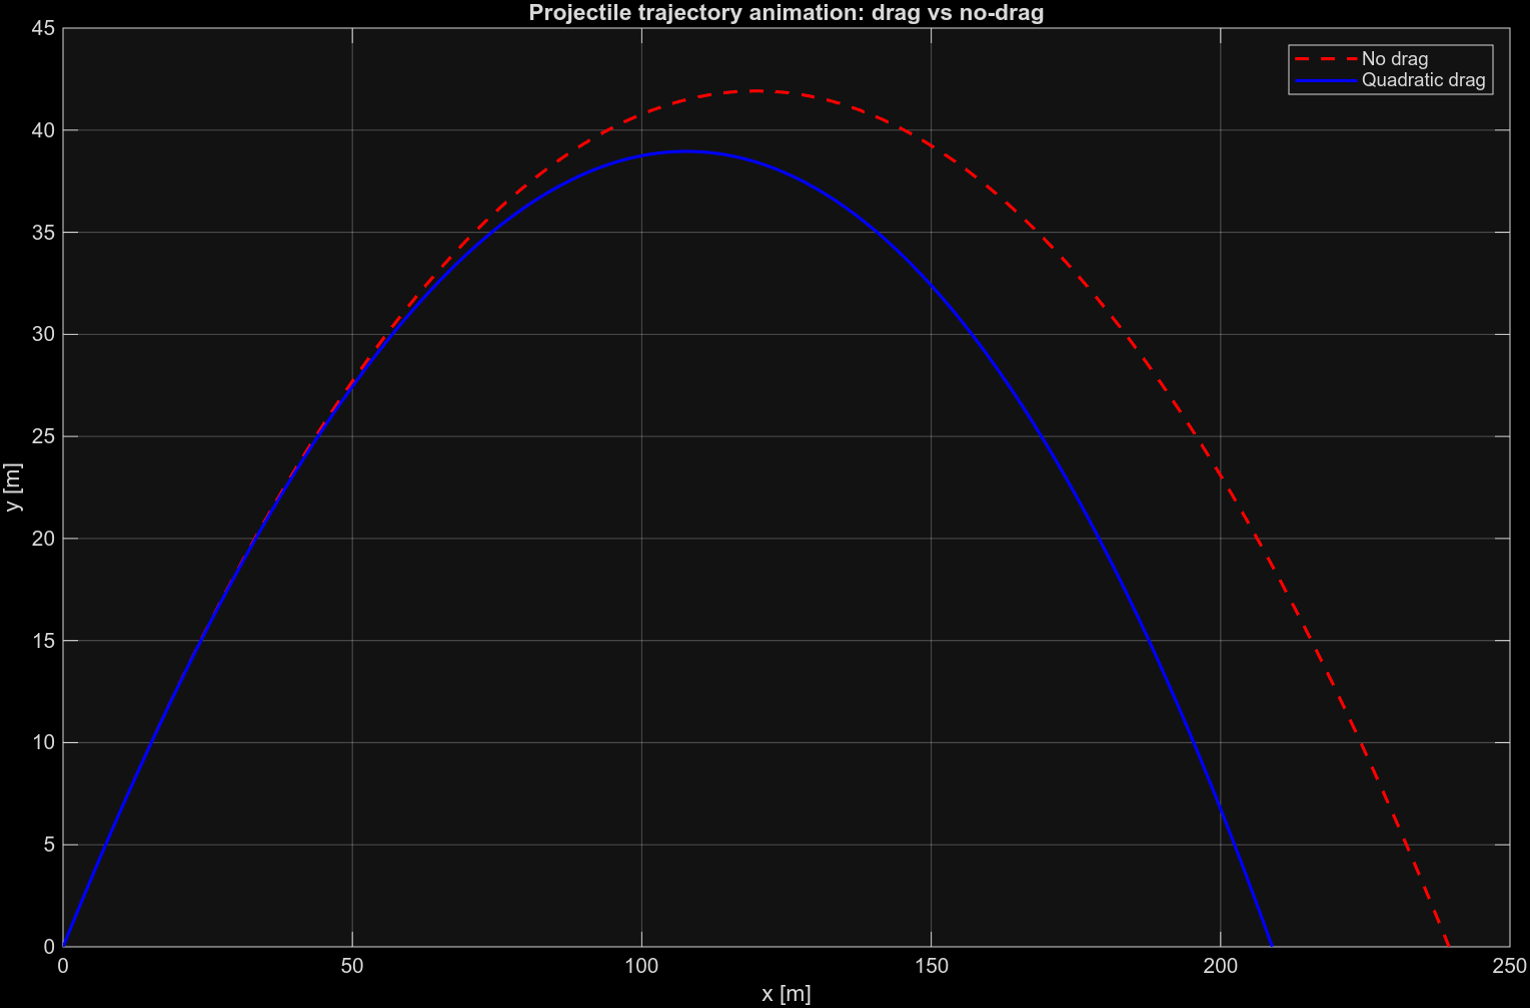
\includegraphics[width=0.8\textwidth]{~/myproject/projectile_drag/results/Trajectory.png} % path to your saved PNG
    \caption{Comparison of projectile trajectories: red dashed = no drag, blue solid = quadratic drag. Drag reduces the range and maximum height.}
    \label{fig:trajectory}
\end{figure}

\subsection{Observations}
\begin{itemize}
    \item Maximum range decreases from 238~m (no drag) to 146~m (with quadratic drag).
    \item Maximum height is also reduced.
    \item Flight time slightly decreases due to drag.
\end{itemize}

\section{Discussion}
The results highlight the importance of drag in real-world projectile motion. Even a modest drag coefficient ($C_D = 0.1$) significantly shortens the range and reduces height. This demonstrates why neglecting air resistance in practical applications can lead to overestimations.

\section{Conclusion}
Numerical simulations confirm the theoretical expectations: drag reduces the projectile's range and height. The MATLAB simulation provides a flexible tool to visualize and quantify these effects.

\section{References}
\begin{itemize}
    \item Morin, D., \emph{Introduction to Classical Mechanics}, Cambridge University Press, 2008.
    \item Kreyszig, E., \emph{Advanced Engineering Mathematics}, 10th Edition, Wiley, 2011.
\end{itemize}

\end{document}
